\section{The C++ standard library}
\begin{frame}
  \frametitle{What is the standard library?}
  The standard library is the set of components specified by the ISO C++ standard ($\sim 1600$ dense pages for C++17) and shipped with identical behavior (modulo performance) by every C++ implementation.
  \vfill
  \url{https://github.com/cplusplus/draft}
\end{frame}
\subsection{Summary}
\begin{frame}
  \frametitle{The C++ Programming Language}
  \centering
  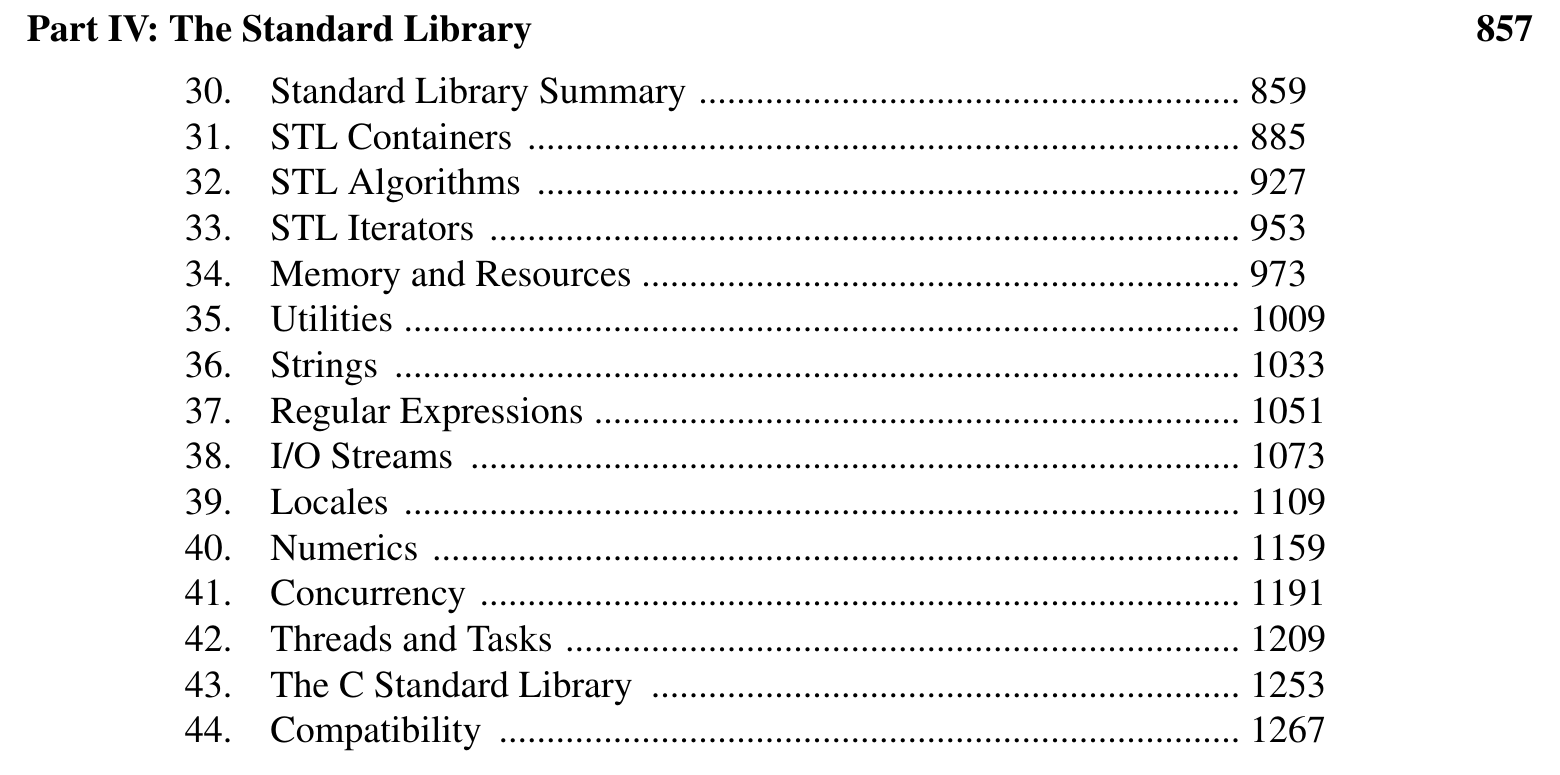
\includegraphics[height=0.7\textheight]{img/summary.png}
\end{frame}

\subsection{Headers}
\begin{frame}
  \frametitle{The header files}
  \centering
  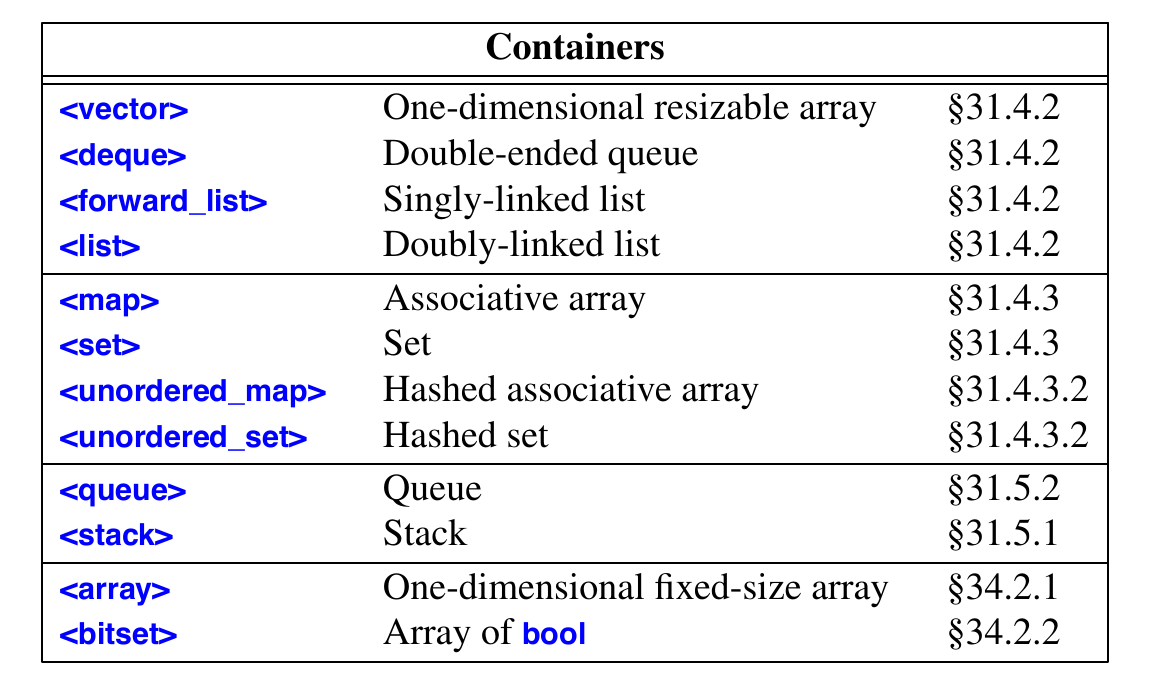
\includegraphics[width=0.7\textwidth]{img/head_01.png}
\end{frame}
\begin{frame}
  \frametitle{The header files}
  \centering
  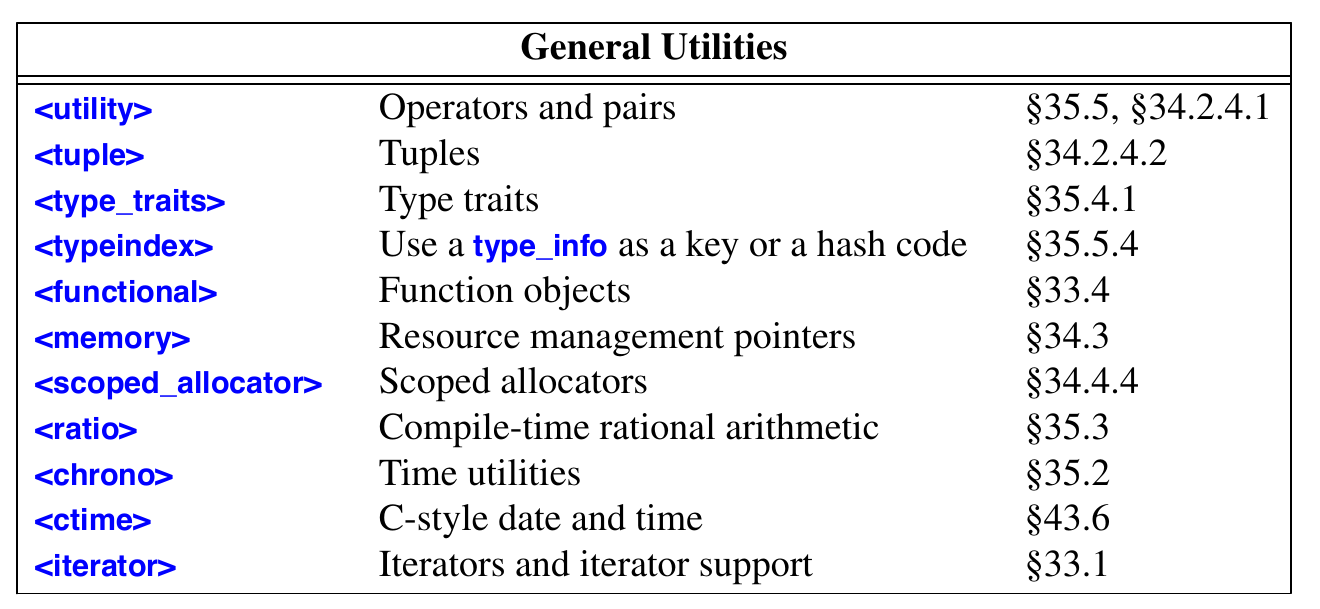
\includegraphics[width=0.7\textwidth]{img/head_02.png}
\end{frame}
\begin{frame}
  \frametitle{The header files}
  \centering
  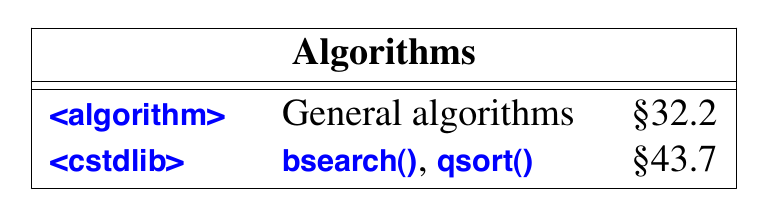
\includegraphics[width=0.7\textwidth]{img/head_03.png}
\end{frame}
\begin{frame}
  \frametitle{The header files}
  \centering
  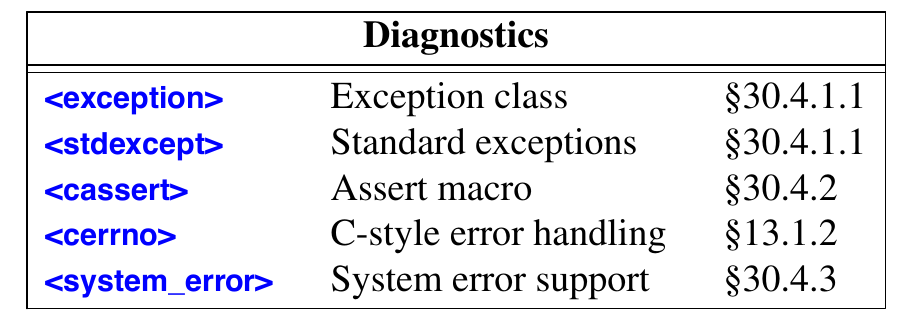
\includegraphics[width=0.7\textwidth]{img/head_04.png}
\end{frame}
\begin{frame}
  \frametitle{The header files}
  \centering
  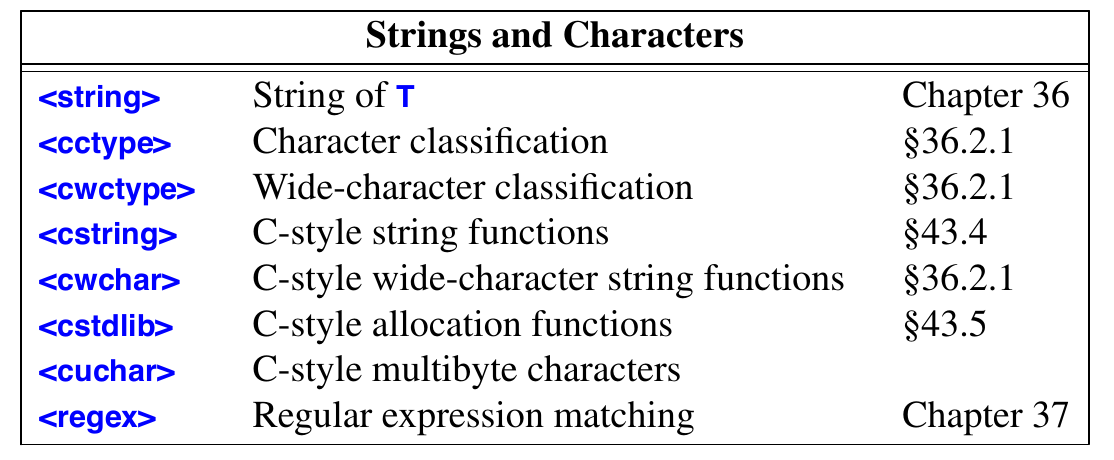
\includegraphics[width=0.7\textwidth]{img/head_05.png}
\end{frame}
\begin{frame}
  \frametitle{The header files}
  \centering
  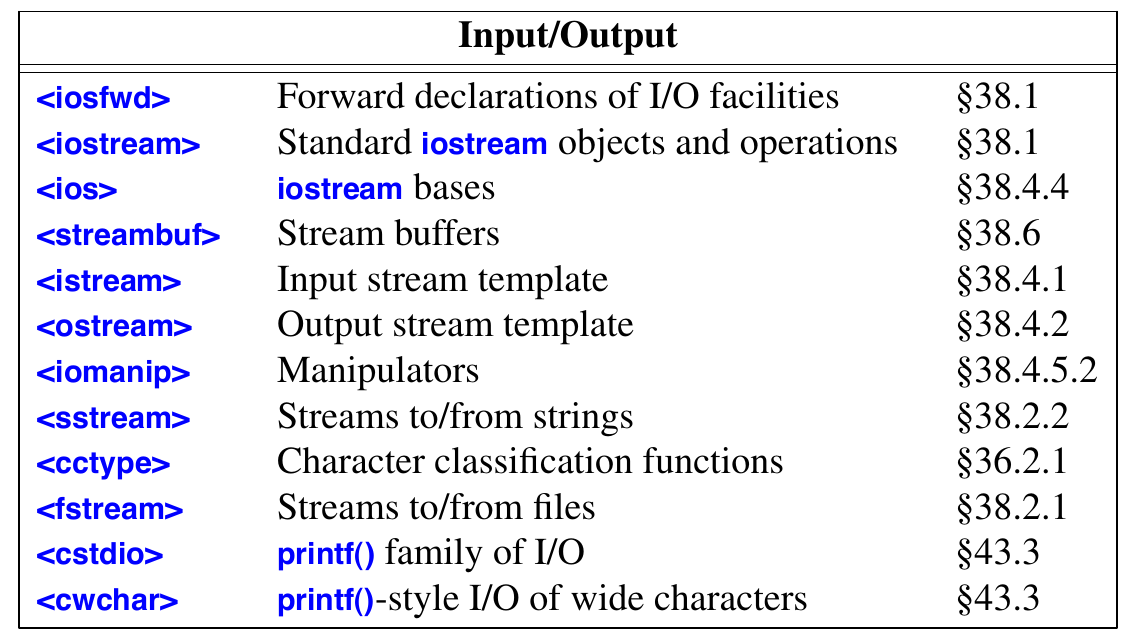
\includegraphics[width=0.7\textwidth]{img/head_06.png}
\end{frame}
\begin{frame}
  \frametitle{The header files}
  \centering
  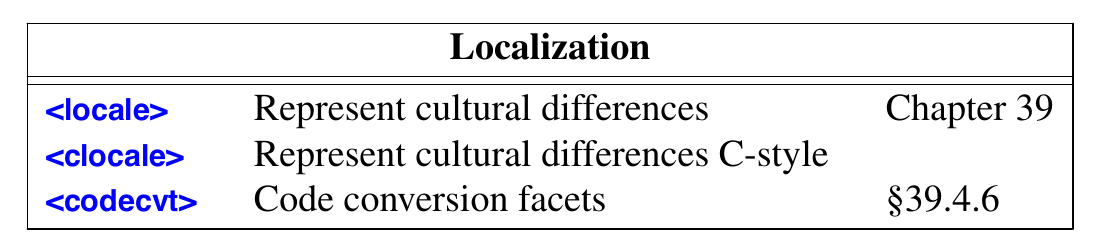
\includegraphics[width=0.7\textwidth]{img/head_07.png}
\end{frame}
\begin{frame}
  \frametitle{The header files}
  \centering
  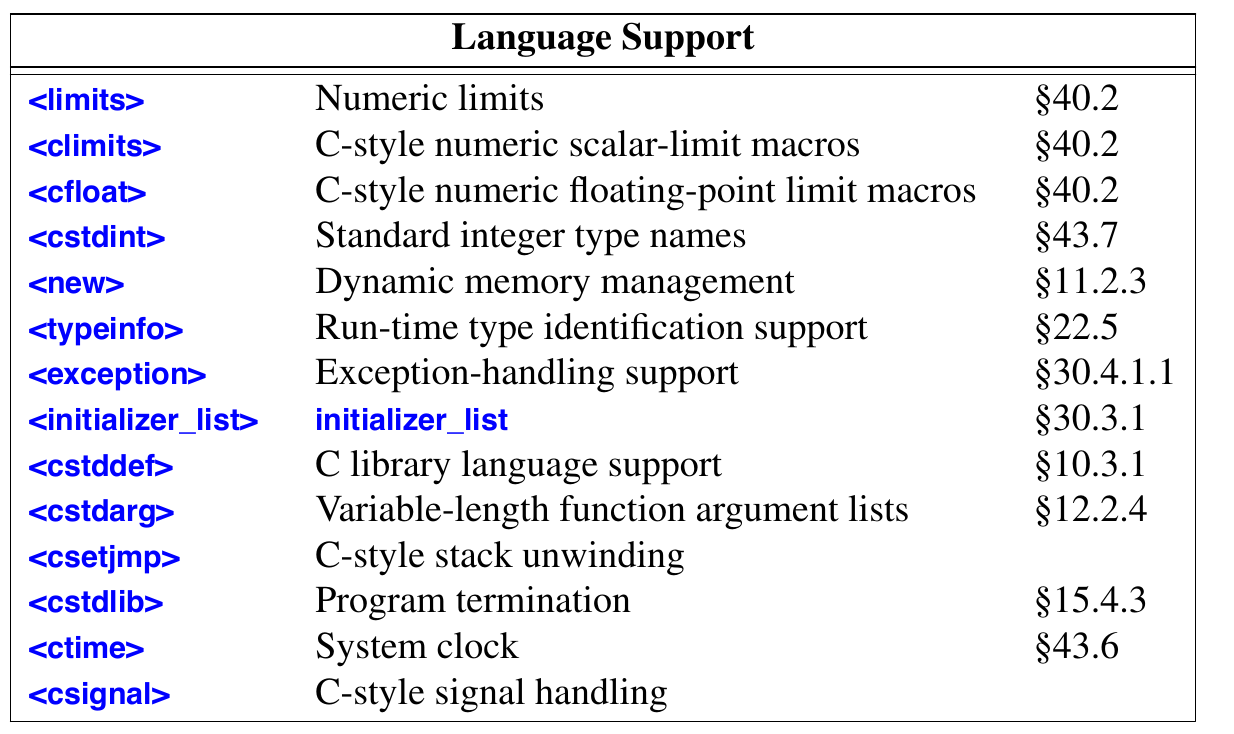
\includegraphics[width=0.7\textwidth]{img/head_08.png}
\end{frame}
\begin{frame}
  \frametitle{The header files}
  \centering
  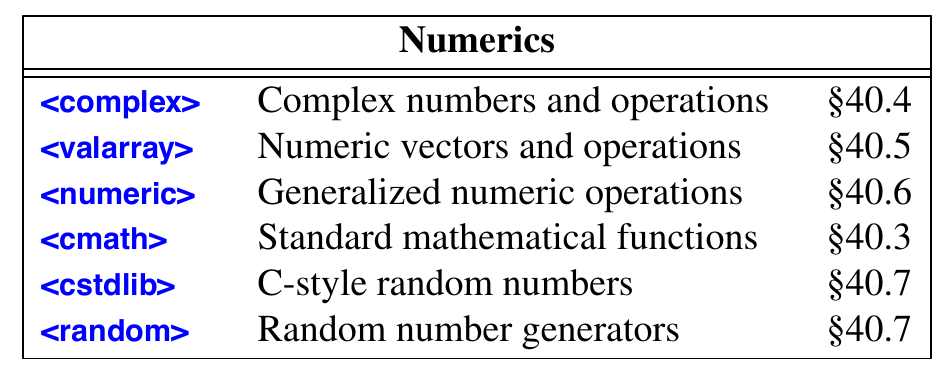
\includegraphics[width=0.7\textwidth]{img/head_09.png}
\end{frame}
\begin{frame}
  \frametitle{The header files}
  \centering
  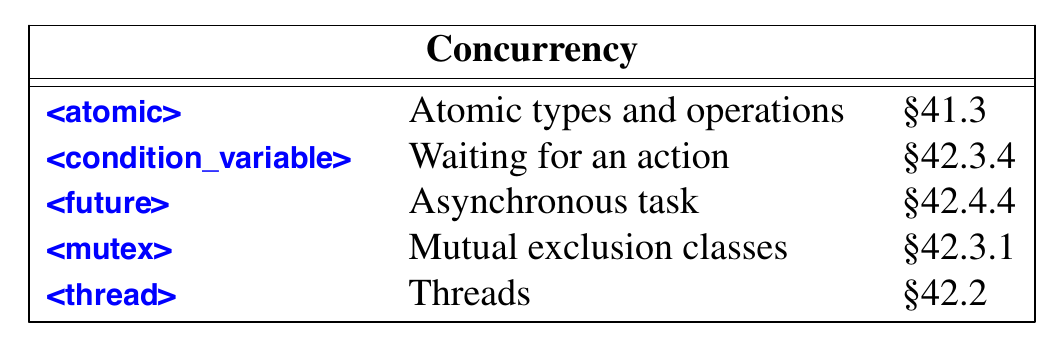
\includegraphics[width=0.7\textwidth]{img/head_10.png}
\end{frame}
\begin{frame}
  \frametitle{The header files}
  \centering
  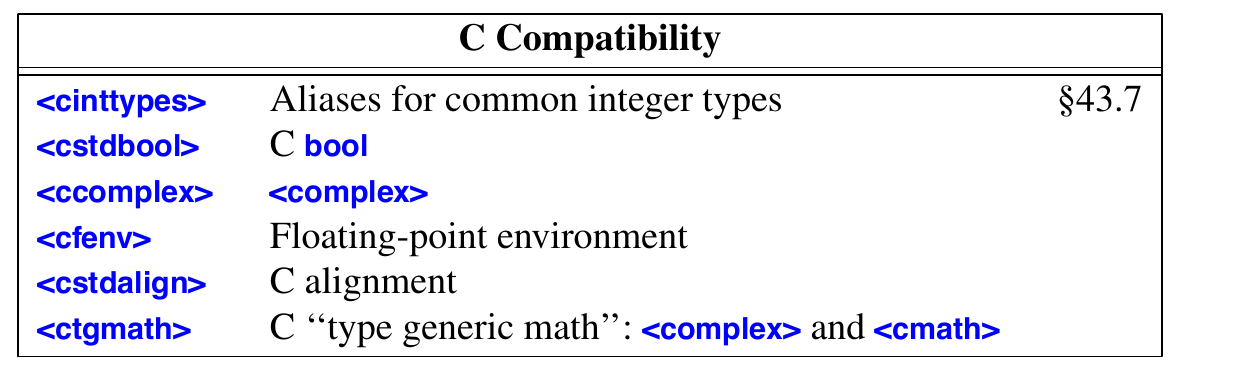
\includegraphics[width=0.7\textwidth]{img/head_11.png}
\end{frame}
\begin{frame}
  \frametitle{The header files}
  \centering
  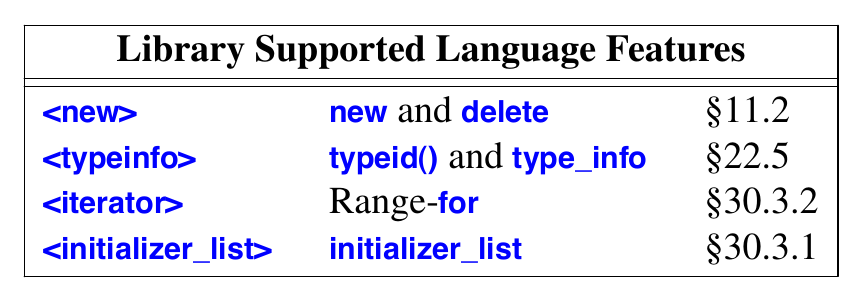
\includegraphics[width=0.7\textwidth]{img/head_12.png}
\end{frame}
\subsection{STL}
\begin{frame}
  \frametitle{We will focus on the STL \smiley}
  \centering
  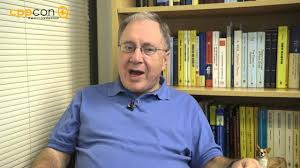
\includegraphics[width=0.6\textwidth]{img/alex.jpeg}
  \hfill
  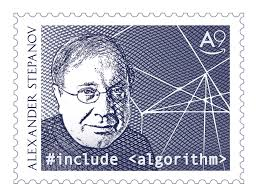
\includegraphics[width=0.35\textwidth]{img/alex2.jpeg}
  \hfill
\end{frame}
\subsection{Concurrency}
\begin{frame}[fragile]
  \frametitle{We will not see the concurrency library \frownie }
\begin{lstlisting}
  int main(){
    // f and g are independent
    f();
    g();
  }
\end{lstlisting}
\end{frame}

\begin{frame}[fragile]
  \frametitle{We will not see the concurrency library  \frownie }
\begin{lstlisting}
  #include <thread>
    
  int main(){
    // f and g are independent
    std::thread t{ f };
    g();
    t.join();
  }
\end{lstlisting}

\end{frame}



\begin{frame}[fragile]
  \frametitle{We will not see the concurrency library \frownie }
\begin{lstlisting}
  #include <future>
    
  int main(){
    // f and g are independent
    auto from_f = std::async( f );
    auto from_g = g();
    ...
    complicated( from_g, from_f.get() );
  }
\end{lstlisting}
\end{frame}

\begin{frame}[fragile]
  \frametitle{We will not see the concurrency library \frownie }
  \framesubtitle{Link  against \texttt{pthread}}
%% \lstset{language=bash}
\begin{lstlisting}
  $ c++ test.cpp -pthread
\end{lstlisting}
\vfill
\begin{lstlisting}
  $ c++ test.cpp -c
  $ c++ test.o -pthread
\end{lstlisting}

\end{frame}
